\documentclass{article}
\usepackage{amsmath}
\usepackage{amssymb}
\usepackage{graphicx}
\usepackage{hyperref}
\usepackage[version=4]{mhchem}

\title{Problem 2}
\date{}

\begin{document}
\maketitle

\section*{Problem}
As shown in the figure, in triangle \(A B C\), median \(B D\) intersects \(C F\) at \(E\) such that \(B F=4\) and \(B E=E D\). Find the length of \(B A\).\\
\centering
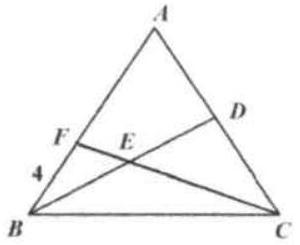
\includegraphics[width=\textwidth]{images/126(2).jpg}

\section*{Solution}
12.\\
Method 1:\\
Draw \(D G / / A B\) to meet \(C F\) at \(G\). Since \(D\) is the midpoint of \(A C\), \(A F=2 D G\).\\
\centering
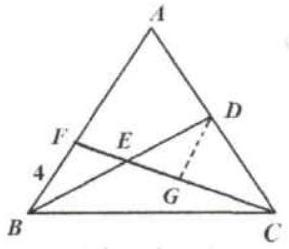
\includegraphics[width=\textwidth]{images/131(1).jpg}


Since \(B E=E D, \angle E B F=\angle E D G\) (alternate interior angles) and \(\angle B E F=\angle D E G\) (vertical angles), \(\triangle E F B \cong \triangle E G D\) and \(D G=B F=4 . A F=2 D G=8 . A B=4+8=\) 12.

Method 2:\\
Pick up a point \(G\) on \(E C\) such that \(F E=E G\). Connect \(D\) with \(G\).\\
Since \(F E=E G\) and \(B E=E D\) (diagonal bisects each other), \(F D G B\) is a parallelogram. Thus \(D G=4, A F=8, A B=12\).\\
\centering
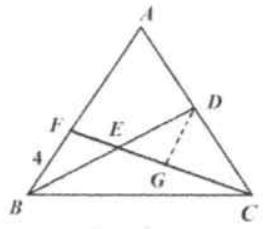
\includegraphics[width=\textwidth]{images/132(1).jpg}

\end{document}
